%% This is file `elsarticle-template-3-num.tex',
%%
%% Copyright 2009 Elsevier Ltd
%%
%% This file is part of the 'Elsarticle Bundle'.
%% ---------------------------------------------
%%
%% It may be distributed under the conditions of the LaTeX Project Public
%% License, either version 1.2 of this license or (at your option) any
%% later version.  The latest version of this license is in
%%    http://www.latex-project.org/lppl.txt
%% and version 1.2 or later is part of all distributions of LaTeX
%% version 1999/12/01 or later.
%%
%% given in the file `manifest.txt'.
%%
%% Template article for Elsevier's document class `elsarticle'
%% with numbered style bibliographic references
%%
%% $Id: elsarticle-template-3-num.tex 165 2009-10-08 07:58:10Z rishi $
%% $URL: http://lenova.river-valley.com/svn/elsbst/trunk/elsarticle-template-3-num.tex $
%%
%\documentclass[preprint,12pt]{elsarticle}

%% Use the option review to obtain double line spacing
%% \documentclass[preprint,review,12pt]{elsarticle}

%% Use the options 1p,twocolumn; 3p; 3p,twocolumn; 5p; or 5p,twocolumn
%% for a journal layout:
%% \documentclass[final,1p,times]{elsarticle}
%% \documentclass[final,1p,times,twocolumn]{elsarticle}
%% \documentclass[final,3p,times]{elsarticle}
%% \documentclass[final,3p,times,twocolumn]{elsarticle}
\documentclass[final,5p,times]{elsarticle}
%% \documentclass[final,5p,times,twocolumn]{elsarticle}

%% if you use PostScript figures in your article
%% use the graphics package for simple commands
%% \usepackage{graphics}
%% or use the graphicx package for more complicated commands
 \usepackage{graphicx}
%% or use the epsfig package if you prefer to use the old commands
%% \usepackage{epsfig}

%% The amssymb package provides various useful mathematical symbols
\usepackage{amssymb}
\usepackage{amsmath}
%% The amsthm package provides extended theorem environments
%% \usepackage{amsthm}

%% The numcompress package shorten the last page in references.
%% `nodots' option removes dots from firstnames in references.
\usepackage[nodots]{numcompress}

%% The lineno packages adds line numbers. Start line numbering with
%% \begin{linenumbers}, end it with \end{linenumbers}. Or switch it on
%% for the whole article with \linenumbers after \end{frontmatter}.
\usepackage{lineno}

%% Avoids linenumbers to collide with text for 5p format:
\setlength\linenumbersep{3pt}

%% natbib.sty is loaded by default. However, natbib options can be
%% provided with \biboptions{...} command. Following options are
%% valid:

%%   round  -  round parentheses are used (default)
%%   square -  square brackets are used   [option]
%%   curly  -  curly braces are used      {option}
%%   angle  -  angle brackets are used    <option>
%%   semicolon  -  multiple citations separated by semi-colon
%%   colon  - same as semicolon, an earlier confusion
%%   comma  -  separated by comma
%%   numbers-  selects numerical citations
%%   super  -  numerical citations as superscripts
%%   sort   -  sorts multiple citations according to order in ref. list
%%   sort&compress   -  like sort, but also compresses numerical citations
%%   compress - compresses without sorting
%%
%% \biboptions{comma,round}

% \biboptions{}


\journal{Computers \& Graphics}

\begin{document}

\begin{frontmatter}

%% Title, authors and addresses

%% use the tnoteref command within \title for footnotes;
%% use the tnotetext command for the associated footnote;
%% use the fnref command within \author or \address for footnotes;
%% use the fntext command for the associated footnote;
%% use the corref command within \author for corresponding author footnotes;
%% use the cortext command for the associated footnote;
%% use the ead command for the email address,
%% and the form \ead[url] for the home page:
%%
%% \ title{Title\tnoteref{label1}}
%% \tnotetext[label1]{}
%% \ead{email address}
%% \ead[url]{home page}
%% \fntext[label2]{}
%% \cortext[cor1]{}
%% \address{Address\fnref{label3}}
%% \fntext[label3]{}

\title{Procedural Bread Making}

%% use optional labels to link authors explicitly to addresses:
%% \author[label1,label2]{<author name>}
%% \address[label1]{<address>}
%% \address[label2]{<address>}

\author{}

\address{}

\begin{abstract}
%% Text of abstract

\end{abstract}

\begin{keyword}
%% keywords here, in the form: keyword \sep keyword

%% MSC codes here, in the form: \MSC code \sep code
%% or \MSC[2008] code \sep code (2000 is the default)

\end{keyword}

\end{frontmatter}

%%
%% Start line numbering here if you want
%%
\linenumbers

%% main text
\section{Introduction}


\section{Previous Work}
Accurate geometry models represents a main requirement in material modeling and rendering \cite{Dorsey2007}. Geometric modeling of structures requires a large amount of information, and artists do most of the work in certain cases.

Procedural modeling avoids the need for artistic intervention in large domains and is also useful when a mathematical description is possible. It is necessary when the problem scale exceeds certain limits: cities \cite{Parish2001}, planets \cite{Ebert2002}, buildings \cite{Muller2006}, and plants \cite{Prusinkiewicz1990}. They define mathematical geometry descriptions using grammars showing the relationship between primitives such as cubes, cilynders and lines. The final structure emerges when grammar elements represents the original structure, in other words, using recursion.

In addition, complex mathematical models represents the behaviour and growing of several natural phenomena. In computer graphics, some work used them to model water and fluids \cite{Stam1999,Fedkiw2001}. Authors borrow differential equations from other science fields and approximate them using numerical techniques. In recent years, GPGPU technology \cite{Owens2007} made them available for use at interactive or real time rates.

In bread modeling, the rendering stage also presents a challenge since it shows complex light phenomena: self-occlusion, self-shadowing, transmittance and reflection, among others. Some studies introduced complex solutions for its rendering \cite{Tong2005}. Nevertheless, such procedures need a complex equipment and set up, limiting the result to one capture. 

In this type of material, it is crucial to simultaneously generate an accurate geometry model and represent the material's light interaction. Literature shows only a few approaches to manage both situations using artistical considerations \cite{Cho2007}. Nevertheless, the authors did not publish enough details of the model and rendering since a private movies company developed the method. A previous work applied a mathematical model of baking to certain types of bread for rendering animations \cite{Rodriguez-Arenas2011}, but they did not show the breads' bubble interior.

To gain modeling flexibility, literature shows methods for geometrical deformations \cite{Lipman2008,Floater2003}. These techniques uses cages with user defined control points to perform deformations. Changing the control points, it is possible to perform natural animations using only one geometry, allowing artists to participate in the process.

Here we propose to unify the key steps of bread making (proving, baking, human deformation) to produce a physically correct pipeline for procedural generation of bread crumb geometries. Using this approach, we follow the ideas of Predictive Rendering \cite{Wilkie2009}, using mathematical models to make physically correct simulations. Next section introduces this model.

\section{Bread making algorithm}

\begin{figure}
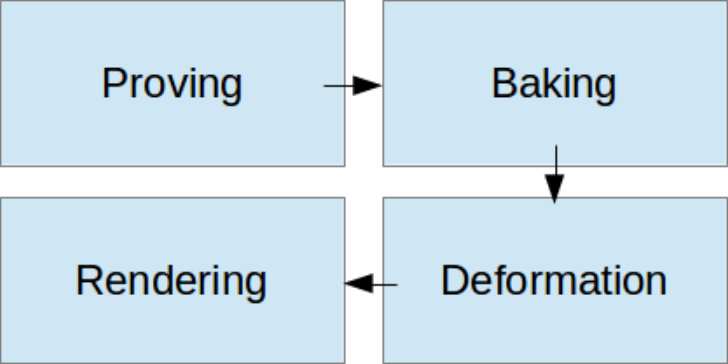
\includegraphics[scale=0.45]{pipeline.png}
\caption{Pipeline for synthetic bread making.}
\label{FigPipeline}
\end{figure}

Fig~\ref{FigPipeline} outlines our model's  pipeline. It consists of $4$ sequential stages emulating bread making. The first step introduces an algorithm for bread proving simulation. Then we apply the bread baking mathematical model \cite{Powathil2004} to slightly deform the bubbles. The third step employs Mean Value Coordinates (MVC) \cite{Floater2003} for an user defined warping of the resulting structure. Finally we apply direct volume rendering getting realistic images of the process.

The proving step is defined in a $3D$ cube. We apply the baking and deformation steps to resulting $2D$ volume slices, since the baking model is cilyndrical (the properties are constant in the $Z$ coordinate).


The next subsection shows the first stage of this pipeline.

\subsection{Proving simulation}
\label{breadprov}
Bubble patterns in bread result from complex processes: chemical reactions and physical deformations in bread dough. Bread making involves two sequential sub-processes: {\em proving} \cite{Babin2006} and {\em baking} \cite{Mondal2008}. Proving accounts for free bubble growth produced by living yeast in dough. Then, human intervention deforms dough shapes in several ways. The baking process gives the final bubbles' shape.

Phenomenological studies of bubble distribution employed X-ray tomography devices and image feature extraction \cite{Babin2006, VanDyck2014,  Gonzales2008}. Despite its accuracy, this method fixs the structure with the capture.

To obtain structure variability, we generate bubbles distributions with a fractal-based model \cite{Mandelbrot1982} and we validate them using the multifractal spectrum \cite{Xu2009}.

\paragraph{Fractal bubble distribution}
Literature shows that the proving stage of bread making strongly determines bubble distributions in bread crumbs \cite{Babin2006}. In this step, interaction between the yeast and the dough produces {\em $CO_{2}$}. Bubble radius differs in the dough, making it a fractal-like structure. Studies computed different fractal dimensions of these structures for certain bread types \cite{Gonzales2008} , suggesting a fractal bubble distribution. We employ this idea to generate different radius for the bubbles.

In addition, direct examination of binarised bread crumb images (see Fig~\ref{FigRealBinarisation}) reveals similarities with certain fractal structures. Previous studies in fractals proposed a model to capture natural phenomena such as moon craters and bubble size distribution in cheeses \cite{Mandelbrot1982}. The author defines radius for circles subtracting them from a white image using the relationship $r = Q/\sqrt{p}$, where $p$ is a random natural number, $r$ is the radius of the subtracted circle and $Q$ is a parameter determining the fractal dimension of the remaining image (the black region). This fractal dimension is equal to $2-2\pi Q^{2}$.

We introduce a model in space using these ideas. We start with an sphere with initial radius of $1$ voxel and then we increment it. The number of spheres extracted in each step is proportional to the radius in the following way:

\begin{equation}
num\_spheres = c/r^{d},
\end{equation}

\noindent where $k$ is a real-value parameter, $r$ is the sphere radius, and $d$ = 3. Fig.~\ref{FigProving} shows a $2D$ example of our model.  The relationship establishes that the number of extracted spheres decreases when the radius increases. We use $k$ to control the amount of spheres we introduce in each step.

We employed different values for k obtaining similar results if $3=<d<=4$. Images show high size distribution resemblance with real bread binarisations (see Fig~\ref{FigBreadbin}). Next subsection explains the application of the bread baking process to this structure.


\begin{figure}
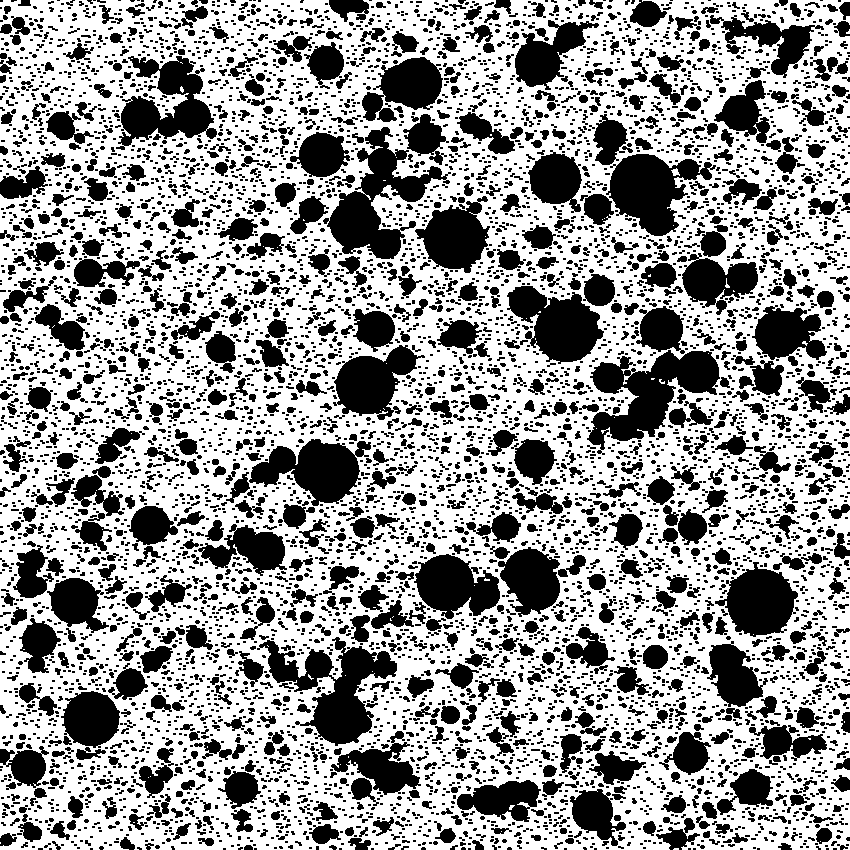
\includegraphics[scale=0.28]{bubbles.png}
\caption{Fractal bread proving simulation.}
\label{FigProving}
\end{figure}

\begin{figure}
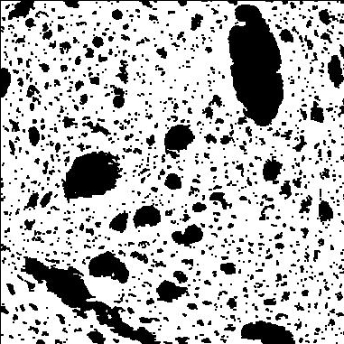
\includegraphics[scale=0.67]{realbin.png}
\caption{Real bread binarisation.}
\label{FigBreadbin}
\end{figure}

\subsection{Baking simulation}
Bread baking mathematical models adequately simulates heat and mass transfer in dough. In our case, a simple one dimensional representation suffices \cite{Powathil2004,Purlis2010}  since the baking effect in bubbles' shape is the lowest in the bread making pipeline. 

We use the numerical implementation in \cite{Powathil2004} that is based on the finite differences scheme. The mathematical model consists of three coupled set of equations describing heat transfer, water vapour diffusion and liquid water diffusion. In our algorithm,  we use only the temperatures ($T$) as the input for the next stage. The next differential equation models heat transfer in bread dough:

\begin{equation}
\frac{\partial T}{\partial t} = \frac{1}{\rho C_{p}} \frac{\partial}{\partial x} \left ( k \frac{\partial T}{\partial x} \right ) + \frac{\lambda}{c_{p}} \frac{\partial W}{\partial t}+\frac{\lambda W}{ C_{p} \rho}\frac{\partial \rho}{\partial t},
\end{equation}


\noindent where $T$ is temperature, $x$ is the space coordinate, $C_{p}$ is the specific heat, $\rho$ is density, $k$ is thermal conductivity and $\lambda$ is the latent heat of evaporation of water. The initial conditions,

\begin{align}
\left ( \frac{\partial T}{\partial x} \right )_{x=L/2} &= 0 , t > 0, \\
T(x,0) &= T_{x}(0), 0\le x \le L/2,\\
\end{align}
and the boundary conditions define the model:
\begin{align}
-k \left ( \frac{\partial T}{\partial x} \right )_{x=0} &= h_{r}(T_{r}-T_{s}) + h_{c}(T_{air}-T_{s}) - \lambda \rho D_{w} \left (\frac{\partial W}{\partial x} \right )_{x=0},
\end{align}

\noindent where $h_{r}$ and $h_{c}$ are subterms of the heat transfer coefficient ($h = h_{r}+h_{c}$), $T_{air}$, $T_{s}$, $T_{r}$ are the temperatures in the surrounding air, at the surface of the bread and at the radiation source, respectively. The model presents similar equations for water vapour diffusion ($W$) and  liquid water diffusion ($V$). Further details of this model can be seen in \cite{Powathil2004}.

The baking simulation sets an oven at $210°C$ and discretises time in intervals of length $\Delta t$.  We obtain an array of $N$ temperature values. Each value represents a dough position after $M$ baking time steps.

We translate this vector into $2D$ coordinates using the following relationship:
\begin{equation}
R = \sqrt{x^{2}+y^{2}},
\end{equation}


\noindent where $R$ is the vector index, and $x$ and $y$ are $2D$ coordinates in the resulting image, {\em i.e.}, we set the image pixel $I(x,y)$ with $v[R]$. Fig.~\ref{FigBakingVectorField} shows rhe result of this process.

We compute a vector field $[g_{x},g_{y}]$ from the image gradient \cite{Gonzalez2006}, and use it to warp the volume texture in the following way:

\begin{eqnarray}
u = x+g_{x}[x,y],\\
v = y+g_{y}[x,y],
\end{eqnarray}
\noindent where $(u,v)$ are the coordinates in the warped image and ($x,y$) are the original image coordinates. Fig.~\ref{FigBakingVectorField} also shows the computed gradient. 


\begin{figure}
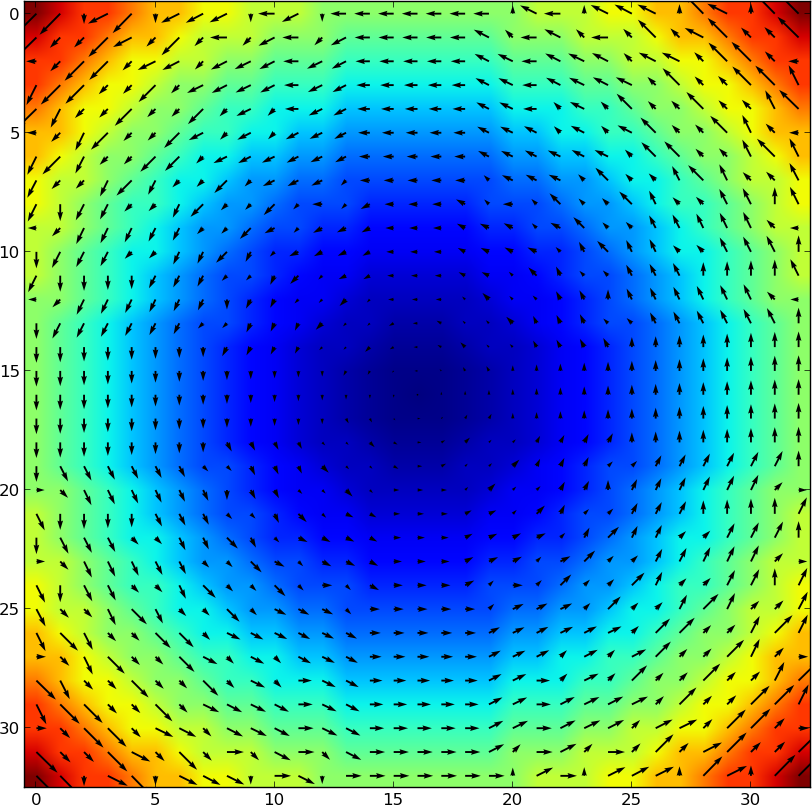
\includegraphics[scale=0.4]{vfield.png}
\caption{Bread baking mathematical model and superimposed gradient vector field .}
\label{FigBakingVectorField}
\end{figure}

Arrow length indicates vector modulus. The image shows that the field's influence is higher near to the crust, mostly deforming outer bubbles. This behaviour is consistent with real bread crumbs: baking influences the outer bubbles' shape, elongating them parallel to the crust \cite{Scanlon2001}.

We warp each volume texture slice, obtaining the final {\em baked} volume. Fig.~\ref{FigBaking} shows a result example of this process.  

\begin{figure}
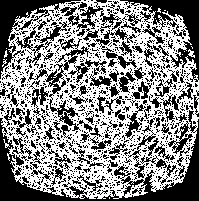
\includegraphics[scale=1.2]{baking.png}
\caption{Volume slice after baking.}
\label{FigBaking}
\end{figure}

Next subsection shows the final texture warping, emulating human intervention in dough.


\subsection{Volume Warping}
In this stage an artist can define control points in an image, changing its external shape to produce natural bread crust silhouettes. 

Mean Value Coordinates (MVC) is a powerful tool for animation \cite{Floater2003,Floater2005,Ju2005}.  This method uses control points to change the structure positions and deforms them using barycentric coordinates.

MVC uses two control points sets for warping. The first one ($cageOrig$) is a point set lying in the original image boundary.  Each texel computes its barycentric coordinates with respect to these points. When we move these points ($cageNew$), the method multiplies the barycentric coordinates with the perturbed control points for each texel:

\begin{align}
barycoords &= MVC([x,y],cageOrig),\\
(u,v) &= \sum {barycoords * cageNew}, \\
T(x,y) &= T(u,v).
\end{align}

Fig.~\ref{FigMVC} shows a warping example using MVC. In that case, $8$ control points were enough to approximate the real crust shape. 

\begin{figure}[ht!]
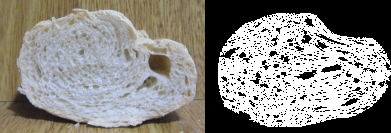
\includegraphics[scale=0.65]{warping.png}
\caption{Image warped using mean value voordinates. The image also shows a real bread image to the left. }
\label{FigMVC}
\end{figure}


This method also warps the bubbles' shape. The deformed bubbles have a natural appearance in concordance with real bread bubbles. 

We apply this step after baking to keep simplicity in the baking step. In real bread making, baking takes place after proving. Our pipeline inverts baking and human deformation. The results we obtained suggests that the inversion produce adequate images for our purposes.

\section{Results}
In this section we present the results of our procedural bread making pipeline and we validate the model using multifractal feature extraction.

\subsection{Rendering}
This step's purpose is the model visualization and image validation.

Direct volume rendering (DVR) \cite{Levoy1988, Max1995,Kruger2003} approximates the *light transfer function* \cite{} by throwing rays into a volume from a virtual camera, accumulating density information. The process forms an image from a camera positioned in space.

We prefer DVR over other state-of-the-art methods such as Ray Tracing \cite{Whitted1980,Singh2010}, Path Tracing \cite{Lafortune1993} and Photon Mapping \cite{Jensen1996}, since they are computationally expensive and they require a detailed object mesh.

Fig.~\ref{FigRenders} shows DVR-rendered images  of the bread making algorithm we presented in this work. Images show a realistic bread crumb appearance, suitable for photo-realistic rendering and serious games \cite{Susi2007}.

\begin{figure}[h!]
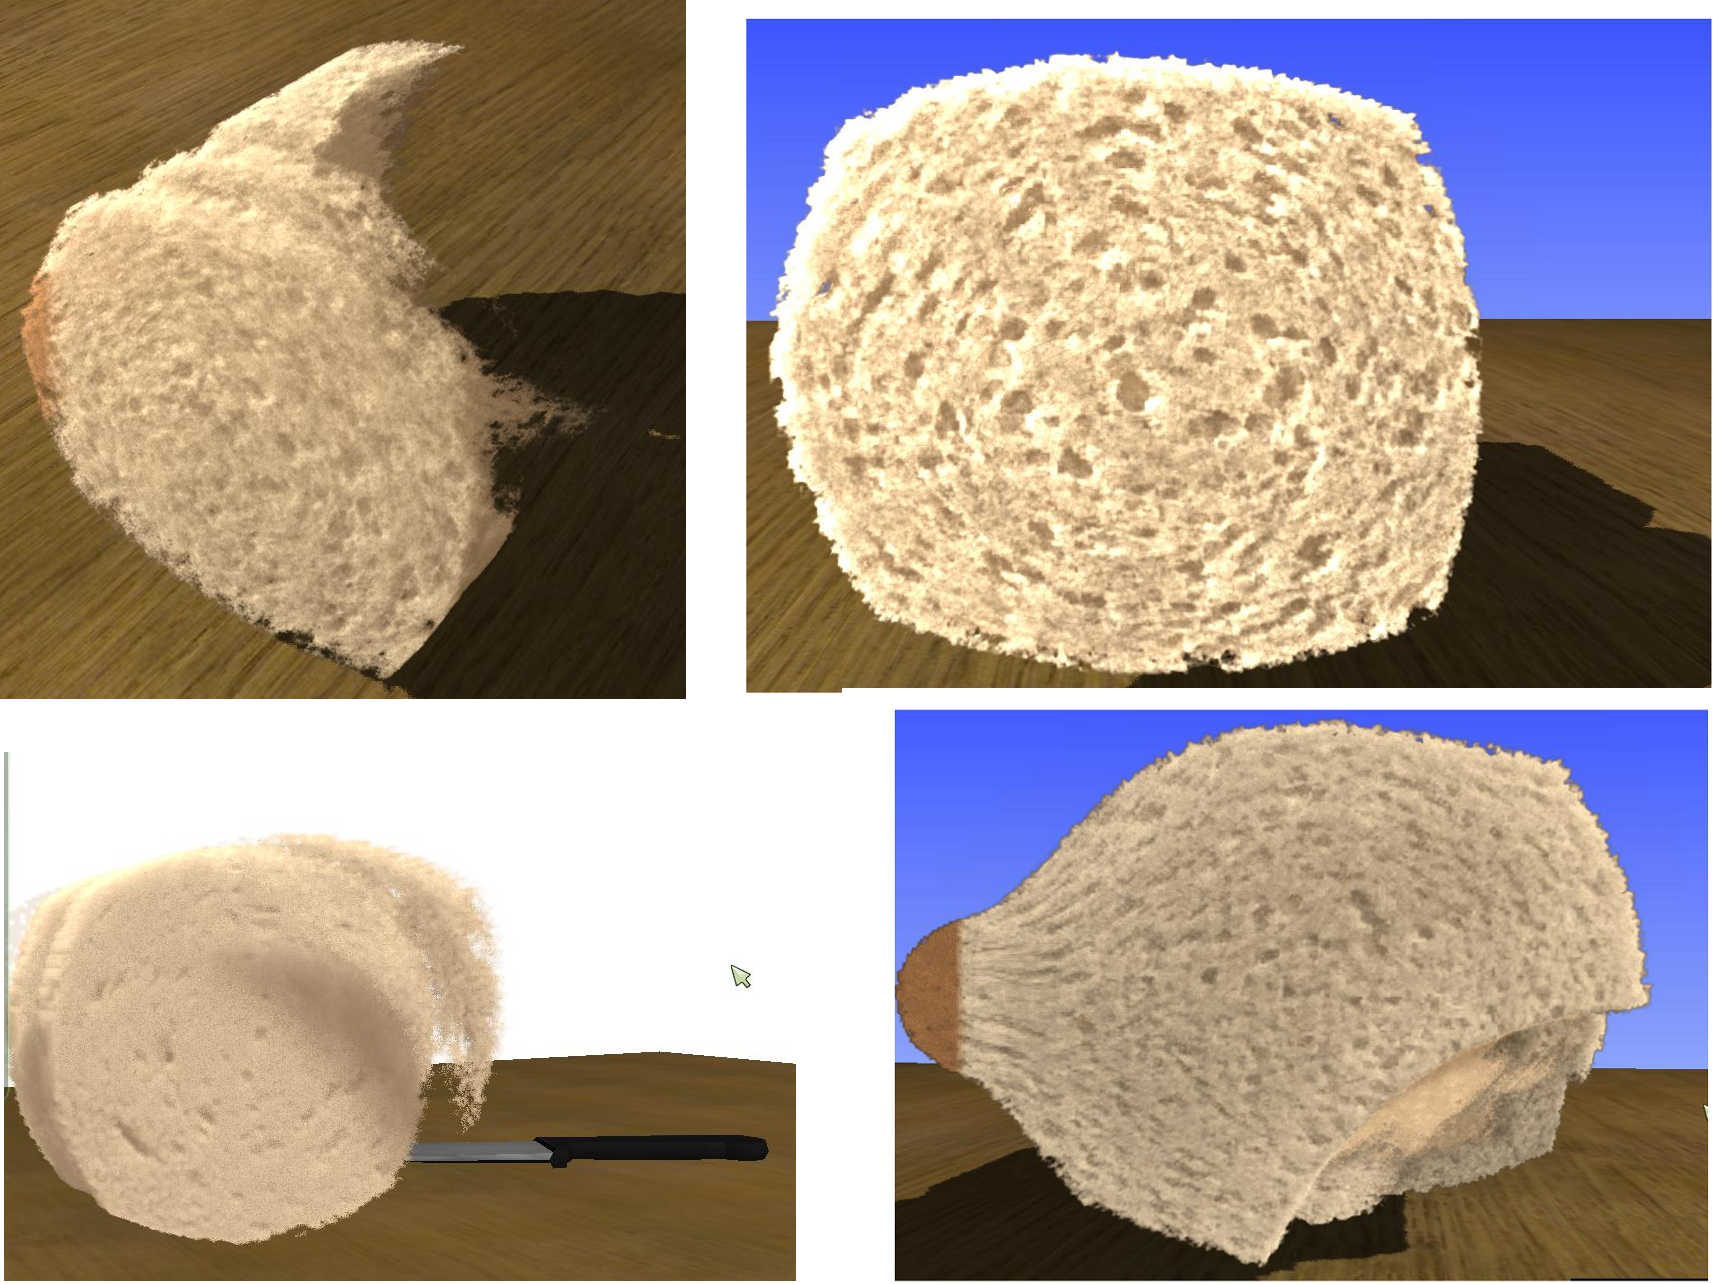
\includegraphics[scale=0.15]{render2.png}
\caption{DVR synthetic bread crumb renders}
\label{FigRenders}
\end{figure}

The authors have used physically correct mathematical models constructing a multi-step pipeline in synthetic bread crumb modelling and visualization. 

Next section validates this model using fractal methods.

\subsection{Model Validation}

Fractal dimensions (FD) measure key image features in narrow representations. Several FDs capture different features, {\em e.g.}, porosity, rugosity, etc.) . Studies shows fractal bread characterisations using several FDs \cite{Gonzales2008,Baravalle2012}. 

We employ the Multifractal Spectrum (MFS) \cite{Xu2009} to validate the model. This method can distinguish bread crumb from non-bread crumb images with high accuracy  \cite{Baravalle2012}.

The MFS applies a pixel based discrimination using pixel neighborhood intensity. The discrimination produces different substructures in the image. The method obtains the Box FD \cite{Peitgen2004} for each structure. This produces a vector of fractal dimensions, {\em i.e.}, different fractals coexists in the structure.
%Similar bubble sizes tends to produce similar pixel characterisations, allowing

SOM maps \cite{Kohonen2001} reduces the N-dimensional feature space into a two dimensional representation while mantaining neighborhood information. These maps allow to see topological relationships among feature vectors.

Fig.~\ref{FigSOM} shows the SOM map for the MFS image representation. We compute the MFS in the $80$ images obtaining a feature vector for each of them. We use these vectors to populate the map. The map we obtained presents evidence for bread and non-bread separability since each class' vectors is separable.

\begin{figure}[h!]
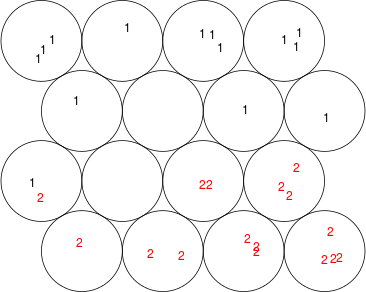
\includegraphics[scale=0.65]{som.png}
\caption{Self Organising Maps showing bread and non-bread separability. 1: Bread, 2: Non-bread }
\label{FigSOM}
\end{figure}

We set a simple experiment to validate synthetic images produced using our method: $20$ real bread crumb images captured with a digital camera and $20$ non-bread images from a public dataset \cite{FeiFei2004} train a Random Forests (RF) \cite{Breiman2001} and Support Vector Machines (SVM) \cite{Vapnik1995} defining $2$ balanced classes. Twenty synthetic images obtained using our method and $20$ non-bread images from the same public dataset defines the test set. We manually segmented real and synthetic bread crumbs to prevent automatic segmentation errors as in \cite{Bosch2011}.


Table~\ref{Table1} shows the classifiers' performance (the percentage of correct classifications in the test set). Table~\ref{Table2} shows the SVM classifier confusion matrix: each row represents the correct class, and each column the classifier result; a diagonal matrix means the classifier performed optimally.

\begin{table}[htb]
\centering
\begin{tabular}{c|c}
\hline
 Method & Accuracy  \\
\hline
 RF & 77.5 \% \\
SVM  & 87.5 \% \\
\hline
\end{tabular}
\caption{Classification performance }
\label{Table1}
\end{table}

\begin{table}[htb]
\centering
\begin{tabular}{c|c|c}
\hline
 Class & bread & non-bread  \\
 \hline
bread & 18 & 2  \\
 non-bread & 3 & 17  \\
 \hline
\end{tabular}
\caption{Confusion matrix for the SVM classifier}
\label{Table2}
\end{table}

\begin{table}[htb]
\centering
\begin{tabular}{c|c|c}
\hline
 Class & bread & non-bread  \\
 \hline
bread & 13 & 7  \\
 non-bread & 2 & 18  \\
 \hline
\end{tabular}
\caption{Confusion matrix for the random forests classifier}
\label{Table3}
\end{table}

An automatic robust classifier classifies most synthetic images as real bread images (the classifiers detected $2$ and $7$ as synthetic). We believe that our procedure adequately models bread crumbs structures. The MFS detects compatible fractal patterns in our synthetic images and in real bread crumbs, suggesting the correctness of the bubble size distributions' model.


%Further research will develop insights on these findings.
%These findings .

%In addition, we compare the Box Dimension of real and synthetic bread crumb images. Box Dimension is a simplification of the Hausdorff (originally Minkowski - Bouligand) dimension for non strictly self-similar objects \cite{Peitgen2004}. The obtained fractal dimensions of real and synthetic images are similar. It means that the space-filling ability of both types of image are comparable.



\section{Discussion}
To the best of the authors' knowledge, this is the first attempt in computer graphics to model the bread crumb geometry using a mathematical model of bread baking and other bread making steps. The problem's complexity, which in certain cases has exceeded available computing capabilities, produced that few work appeared in the literature. With the advenement of GPGPU, more realistic models appeared in other materials. We thought our model may be the first one in a future line of research for bread modeling. 

We proposed and validated a flexible and powerful pipeline to procedurally model bread crumbs. This is a contribution to the state of the art since typical approaches for modeling the geometry of bread crumbs involve advanced tomography equipment \cite{VanDyck2014} or artistical considerations \cite{Cho2007}. The images obtained suggests the correctness of the model, suitable for application in $3D$ engines, serious games and photo-realistic rendering.

Artists can model the bread crumb global shape using control points in a plane. Bubbles naturally follow this shape, accurately emulating bread crumb bubbles.

We employed fractal and machine learning methods to model and validate our procedure. The low error rates we obtained make us beleive that the bubbles' size distribution is accurate in a (multi) fractal sense: the number, sizes and shape of the bubbles concordate with real bread crumbs. Also, since we mathematically emulated key steps in bread making, we obtained natural shapes for bubbles that adapts to the bread exterior silhouette, producing mathematically correct patterns.


\section{Conclusions and future work}

As possible continuations, we will define interfaces for visual interaction with the control points. We plan to perform further tests on our classification procedure to gain insight in bread multi-fractal features.


%% The Appendices part is started with the command \appendix;
%% appendix sections are then done as normal sections
%% \appendix

%% \section{}
%% \label{}

%% References
%%
%% Following citation commands can be used in the body text:
%% Usage of \cite is as follows:
%%   \cite{key}          ==>>  [#]
%%   \cite[chap. 2]{key} ==>>  [#, chap. 2]
%%   \citet{key}         ==>>  Author [#]

%% References with bibTeX database:

\bibliographystyle{model3-num-names}
\bibliography{bib}

%% Authors are advised to submit their bibtex database files. They are
%% requested to list a bibtex style file in the manuscript if they do
%% not want to use model3-num-names.bst.

%% References without bibTeX database:

% \begin{thebibliography}{00}

%% \bibitem must have the following form:
%%   \bibitem{key}...
%%

% \bibitem{}

% \end{thebibliography}


\end{document}

%%
%% End of file `elsarticle-template-3-num.tex'.